\icode{E-MI-SI-L2-261111-001}
如图所示，小球\(A\)和\(B\)的质量均为\(m\)，长度相同的四根细线\(a\)、\(b\)、\(c\)、\(d\)分别连接在两球间、球与水平天花板上\(P\)点以及与竖直墙上的\(Q\)点之间，它们均被拉直，且\(P\)、\(B\)间细线\(c\)恰好处于竖直方向，\(Q\)、\(A\)间水平细线\(b\)恰好处于水平方向，两小球均处于静止状态，则细线\(a\)、\(b\)、\(c\)、\(d\)的拉力大小为\paren[]

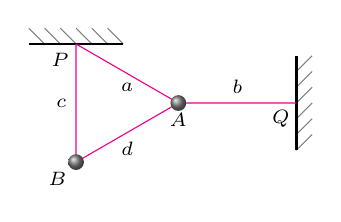
\begin{tikzpicture}[font=\scriptsize]
	\foreach \x in {-.6,-.4,...,.6}
		\draw[gray] (\x,.2)--++(.2,-.2);
	\foreach \y in {-1.35,-1.15,...,-.15}
		\draw[gray] ({.75*sqrt(3)+1.5},\y)--++(.2,.2);
	\draw[thick] (-.6,0)--(.6,0) ({.75*sqrt(3)+1.5},-1.35)--({.75*sqrt(3)+1.5},-.15);
	\coordinate (A) at(-30:1.5);
	\coordinate (Q) at({.75*sqrt(3)+1.5},-.75);
	\coordinate (B) at(0,-1.5);
	\draw[magenta] (0,0)--node[below,black]{\(a\)}(A)--node[above,black]{\(b\)}(Q) (0,0)--node[left,black]{\(c\)}(B)--node[below,black]{\(d\)}(A);
	\shade[ball color=gray] (A)node[below]{\(A\)} circle(.1);
	\shade[ball color=gray] (B)node[below left]{\(B\)} circle(.1);
	\node at(-.2,-.2){\(P\)};
	\node at(2.6,-.95){\(Q\)};
\end{tikzpicture}
\begin{choices}
	\item\(2mg,\sqrt{3}mg,mg,0\)
	\item\(\sqrt{3}mg,mg,\dfrac{1}{2}mg,\dfrac{1}{2}mg\)
	\item\(\dfrac{\sqrt{3}}{3}mg,mg,mg,0\)
	\item\(mg,mg,mg,mg\)
\end{choices}
\begin{answer}
	A\qquad 提示:
\end{answer}